\documentclass{article}
\usepackage[paperwidth=160mm,paperheight=154mm,margin=0pt]{geometry}
\usepackage[UTF8,fontset=none]{ctex}
\IfFontExistsTF{Microsoft YaHei}{%
  \setCJKmainfont{Microsoft YaHei}
  \setCJKsansfont{Microsoft YaHei}
}{%
  \setCJKmainfont{Noto Sans CJK SC}
  \setCJKsansfont{Noto Sans CJK SC}
}
\usepackage{tikz}
\usepackage{graphicx}
\usetikzlibrary{arrows.meta,positioning,calc}
\begin{document}
\pagestyle{empty}\noindent
\begin{tikzpicture}[x=1mm,y=1mm, every node/.style={font=\sffamily}]
\definecolor{ink}{HTML}{272727}
\definecolor{cyan}{HTML}{E0F0F0}
\definecolor{pink}{HTML}{E4CCD8}
\definecolor{green}{HTML}{F0E0D0}
\definecolor{cream}{HTML}{E0E0F0}
\definecolor{blue}{HTML}{0F4D92}
\definecolor{accentred}{HTML}{B64342}
\fill[white] (0,0) rectangle (160,154);
\fill[cyan] (0,113) rectangle (160,154);
\fill[pink] (0,71) rectangle (160,110);
\fill[green] (0,0) rectangle (160,68);
\node[anchor=west,text=ink,font=\sffamily\bfseries\fontsize{12}{14}\selectfont] at (5,148) {问题二  同核Task合并与存储驻留};
\node[anchor=west,text=ink,font=\sffamily\bfseries\fontsize{10}{12}\selectfont] at (5,137) {01 对象与机理};
\node[anchor=west,text=ink,font=\sffamily\fontsize{9}{11}\selectfont] at (6,125) {场景A方案在场景B重新评价};

\draw[rounded corners=1mm,draw=blue!65,fill=white] (72,121) rectangle (111,140);
\draw[rounded corners=1mm,draw=blue!65,fill=white] (117,121) rectangle (156,140);
\node[text=ink,font=\fontsize{8}{9}\selectfont] at (91.5,136) {核心1：单Task};
\node[text=ink,font=\fontsize{8}{9}\selectfont] at (136.5,136) {核心2：单Task};
\node[draw=blue!50,fill=cyan,minimum width=12mm] (b1) at (82,127) {$g_1$};
\node[draw=blue!50,fill=cyan,minimum width=12mm] (b2) at (101,127) {$g_2$};
\node[draw=blue!50,fill=cream,minimum width=12mm] (b3) at (136,127) {$g_3$};
\draw[blue,thick,-{Latex[length=2mm]}] (b1)--(b2);
\draw[accentred,thick,dashed,-{Latex[length=2mm]}] (b2)--node[above,font=\fontsize{7}{8}\selectfont]{COPY}(b3);
\node[text=ink,font=\fontsize{7.3}{8.5}\selectfont] at (113,116) {同核保留；跨核同步与搬运};

\node[anchor=west,text=ink,font=\sffamily\bfseries\fontsize{10}{12}\selectfont] at (5,103) {02 方法与约束};
\node[rounded corners=1mm,draw=blue!50,fill=white,minimum width=43mm,minimum height=19mm,align=center,text=ink,font=\sffamily\fontsize{8.6}{10.5}\selectfont] (a) at (26,89) {同核子图合并\\中间量留在L1/UB};
\node[rounded corners=1mm,draw=blue!50,fill=white,minimum width=43mm,minimum height=19mm,align=center,text=ink,font=\sffamily\fontsize{8.6}{10.5}\selectfont] (b) at (80,89) {跨核边界COPY\\固定同步等待};
\node[rounded corners=1mm,draw=blue!50,fill=white,minimum width=43mm,minimum height=19mm,align=center,text=ink,font=\sffamily\fontsize{8.6}{10.5}\selectfont] (c) at (134,89) {容量约束与Spill\\DDR共享带宽};
\draw[blue,thick,-{Latex[length=2mm]}] (a.east) -- (b.west);
\draw[blue,thick,-{Latex[length=2mm]}] (b.east) -- (c.west);
\node[anchor=west,text=ink,font=\sffamily\fontsize{8.2}{10}\selectfont] at (5,74) {$L(t)\le C_{\rm L1},\;U(t)\le C_{\rm UB}$；按场景B $T_k$ 择优};
\node[anchor=west,text=ink,font=\sffamily\bfseries\fontsize{10}{12}\selectfont] at (5,62) {03 实测结果与核验};
\node[anchor=west,text=ink,font=\sffamily\bfseries\fontsize{8.8}{10.5}\selectfont] at (5,52) {100例五核平均加速比 $3.5456$；同方案A/B比均值 $1.0202$};
\node[anchor=west,text=ink,font=\sffamily\fontsize{8.3}{10}\selectfont] at (5,44) {500个所选配置：合法性与时间线复核；容量峰值取官方输出};
\node[anchor=west] at (5,21) {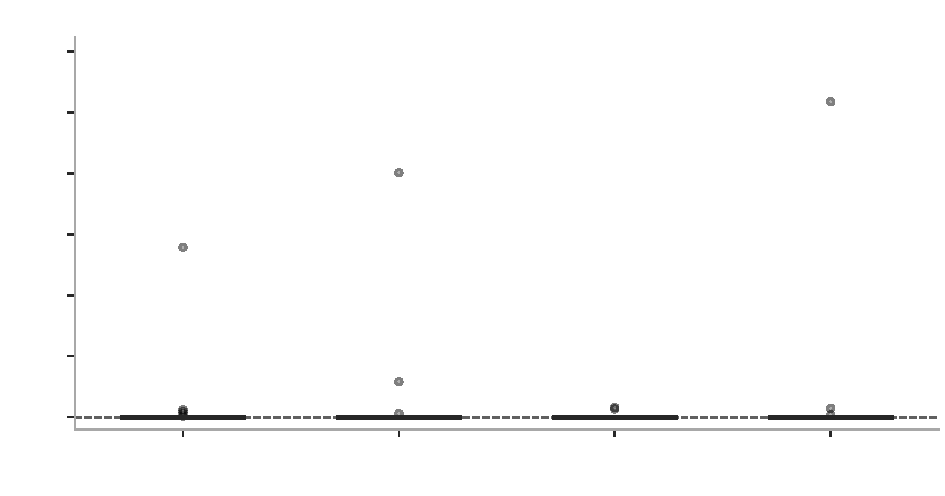
\includegraphics[width=72mm,height=30mm,keepaspectratio]{../正式图件/q2-F02.pdf}};
\node[anchor=east] at (155,21) {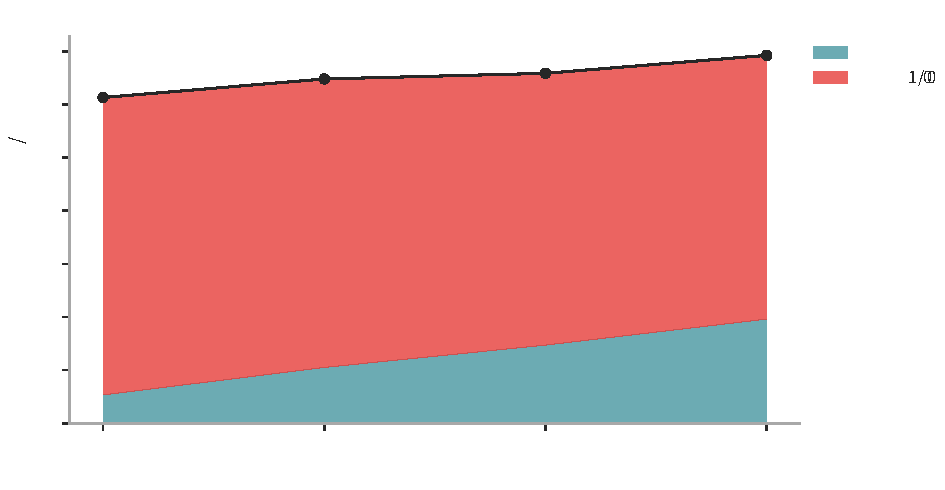
\includegraphics[width=72mm,height=30mm,keepaspectratio]{../正式图件/q2-F03.pdf}};
\node[anchor=west,text=ink,font=\sffamily\fontsize{7.5}{9}\selectfont] at (5,4) {细节参见正文图 q2-F02、q2-F03；缩图仅作证据导航。};
\end{tikzpicture}
\end{document}
